\scanpage{35}
\mspage{27}
% L1–5
\textcircled{\scriptsize\unsure{13}} Cas du \uline{préprisme triangulaire} $D$
\figure{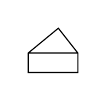
\begin{tikzpicture}[scale=.45]\draw (0,0)--(1.4,0)--(1.4,.55)--(.85,1.25)--(0,.55)--cycle (0,.55)--(1.4,.55);\end{tikzpicture}}
La donnée de ce diagramme dans $C$ équivaut : celle d'un carré
\figure{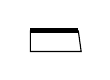
\begin{tikzpicture}[scale=.46]\draw (0,.58)--(0,0)--(1.4,0)--(1.32,.58);\draw[line width=2pt] (0,.58)--(1.32,.58);\end{tikzpicture}}
avec un côté marqué -- on l'étudiera plutôt avec le carré.

% L6–11
\textcircled{\scriptsize\unsure{14}} \unsure{Complexe|Complexes} cubique avec \uline{prisme triangulaire} \inserted{$D_6$} \inserted{ou : \uline{bitriangle} $D_7$}.
\figure{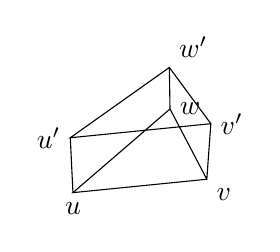
\begin{tikzpicture}[scale=.85]
\coordinate (u) at (0,0); \coordinate (v) at (2,.2); \coordinate (w) at (1.45,1.25);
\coordinate (U) at (-.04,.82); \coordinate (V) at (2.06,1.03); \coordinate (W) at (1.44,1.87);
\draw (u)--(v)--(w)--cycle (U)--(V)--(W)--cycle (u)--(U) (v)--(V) (w)--(W);
\node[below] at (u) {$u$};\node[below right] at (v) {$v$};\node[right] at (w) {$w$};
\node[left] at (U) {$u'$};\node[right] at (V) {$v'$};\node[above right] at (W) {$w'$};
\end{tikzpicture}}
Il donne naissance, en \unsure{fermant|formant} les triangles sur les arêtes latérales, à un bitriangle à paire de triangles \inserted{disjoints} distinguée $\{\{u,v,w\},\{u',v',w'\}\}$ (épinglage partiel).
\figure{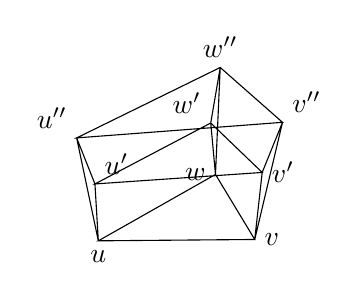
\begin{tikzpicture}[scale=.86]
\coordinate(u) at (.32,0);\coordinate(v) at (2.63,.02);\coordinate(w) at (2.05,.98);
\coordinate(U) at (.27,.84);\coordinate(V) at (2.74,1.01);\coordinate(W) at (1.98,1.74);
\coordinate(A) at (0,1.52);\coordinate(B) at (3.04,1.75);\coordinate(C) at (2.12,2.56);
\draw (u)--(v)--(w)--cycle (U)--(V)--(W)--cycle (A)--(B)--(C)--cycle (u)--(U)--(A)--cycle (v)--(V)--(B)--cycle (w)--(W)--(C)--cycle;
\node[below] at(u){$u$};\node[right] at(v){$v$};\node[left] at(w){$w$};\node[above right] at(U){$u'$};\node[right] at(V){$v'$};\node[above left] at(W){$w'$};
\node[above left] at(A){$u''$};\node[above right] at(B){$v''$};\node[above] at(C){$w''$};
\end{tikzpicture}}

% L12–22
Étudions d'abord les bitriangles, au nb de 120 (cf p. 10) ; \deleted{le gpe des autom d'un diagramme $\Delta$ $(\simeq D_7)$, est \unsure{$\mathfrak S_2$|$\mathfrak G_2$}.} La donnée d'un diagramme de type $D_7$ équivaut : celle d'un ens $\inserted{\Delta_0}$ de cardinal 9, muni de \inserted{un ens $\{\pi,\pi'\}$ de} deux partitions de type $(3,3,3)$, de telle façon que l'application $\Delta_0\unsure{-|\longrightarrow}(\Delta_0/\pi\times\Delta_0/\pi')$ soit bijective, ou encore d'un ens $\inserted{T}$ de cardinal 6 (l'ens des 6 triangles de $\Delta$) et d'une partition de $T$ de type $(3,3)$, i.e. d'une application $T\longrightarrow I$ de degré 3, \deleted{\unsure{cardinal}} $\operatorname{card} I=2$. (\unsure{bon|car}. alors $\Delta_0=\prod_{i\in I}T_i\quad\ldots$) Le gpe des autom
% archive sheet number: 34
